\section{Introduction}
\label{sec:introduction}

LLM-based agents for GPU kernel generation now achieve strong scores on isolated benchmarks~\citep{kernelbench, solexecbench, flashinferbench}, with state-of-the-art systems autonomously compiling, profiling, and refining CUDA or Triton code.
Yet these gains often fail to transfer into production inference frameworks such as vLLM~\citep{vllm} and SGLang~\citep{sglang}: kernels that score well in sandbox evaluation routinely regress once they encounter real serving interfaces, compilation stacks, and workloads.

The root cause is \textbf{benchmark--production misalignment}.
Current benchmarks rely heavily on synthetic inputs, single-GPU isolated kernels, simplified interfaces, and independent task levels that do not compose into full inference pipelines.
They therefore reward kernels that are fast in isolation but brittle in deployed systems, hiding interface mismatches, compilation-stack conflicts, and correctness degradation that only appears at model scale.

\subsection*{Our approach}

We introduce \fastkernels{} (Figure~\ref{fig:overview}), a benchmark for kernel agents designed so that its scores predict deployment outcomes.
\fastkernels{} derives 384 tasks top-down from 47 real model architectures across 8 categories; each task's interface matches the corresponding module in the production library for its family, and each candidate is scored against the kernels that library ships.
Crucially, its task levels are compositional: Level~1 primitives feed Level~2 fused operators, which feed Level~3 layers and Level~4 models.
Unlike benchmarks whose levels are independent, this hierarchy enables a dynamic-programming style optimization loop: an agent can reuse an optimized lower-level kernel, such as a linear operator, when optimizing higher-level modules such as MLPs or transformer blocks, instead of rediscovering the same building block from scratch.

Because integration failures only surface at model scale, \fastkernels{} also scores every candidate end to end, inside the models its tasks come from and on their production execution path (continuous batching, chunked prefill, CUDA graphs, \texttt{torch.compile}, tensor parallelism).
This model runtime is the benchmark's measurement instrument, not a separate contribution, and we validate it against vLLM, SGLang, and the other production references before scoring any agent (Section~\ref{sec:eval-results}).
The result is an open leaderboard that ranks agents by what survives deployment, scored with \textsc{MacroEval}, and we seed it with a 6{,}900-agent-hour evaluation of five representative agents, from an RL-trained kernel model to contest-winning long-horizon harnesses.

\begin{figure*}[t]
\centering
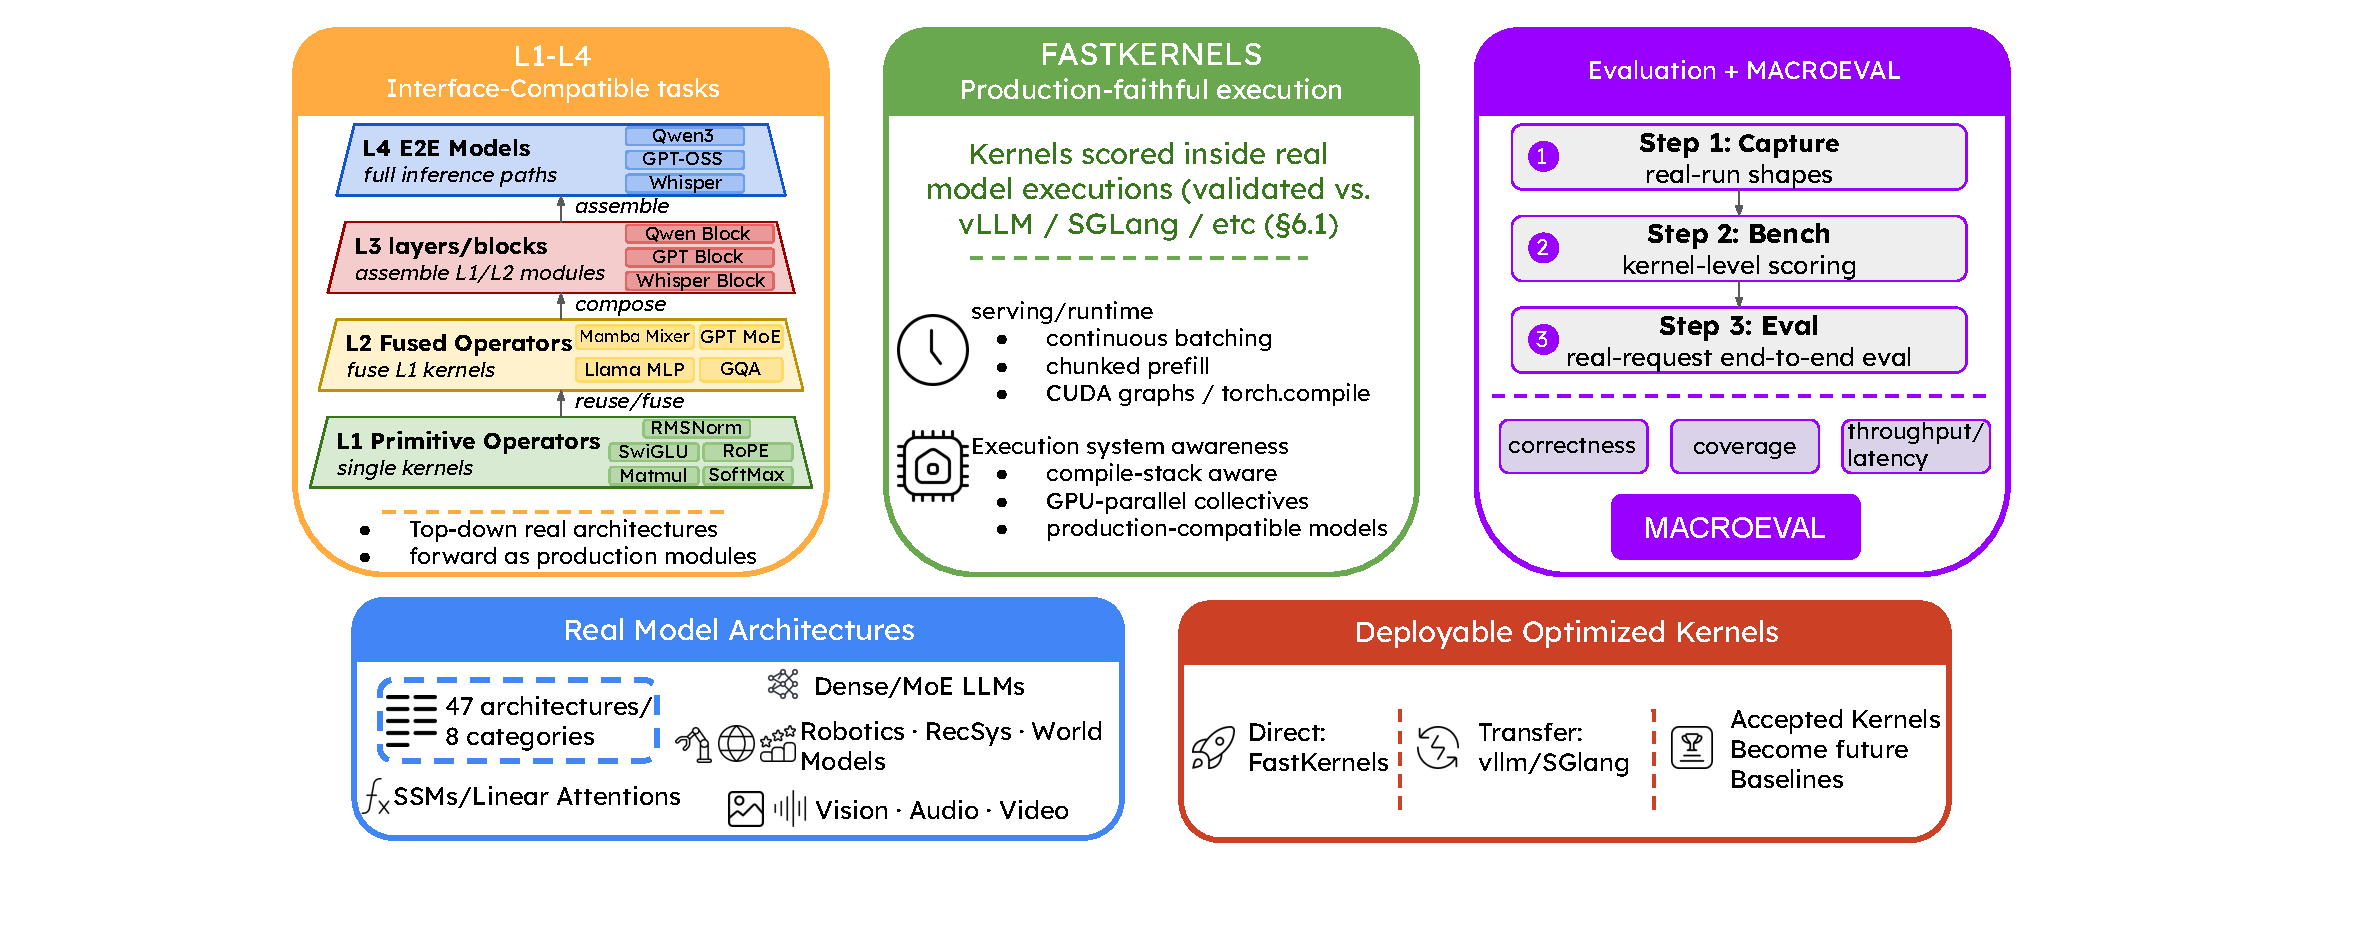
\includegraphics[width=\linewidth]{figures/overview.pdf}
\caption{\textbf{\fastkernels{} overview.} Tasks derived from 47 real architectures (bottom left) form a compositional L1--L4 hierarchy with production interfaces (top left) and run inside validated production model executions (center). Candidates are scored by capture, kernel-level bench, and end-to-end eval, aggregated by \textsc{MacroEval} (right); optimized kernels deploy directly or transfer into vLLM and SGLang (bottom right).}
\label{fig:overview}
\end{figure*}

\subsection*{Contributions}

\begin{enumerate}[leftmargin=*, itemsep=2pt, topsep=2pt]
\item \textbf{Production-aligned task suite.}
384 tasks from 47 architectures across 8 categories, from dense and MoE LLMs and SSMs to vision, audio, robotics, 3D, recommendation, and world models, with production module interfaces and speedups measured against production kernels.

\item \textbf{Compositional task hierarchy.}
Unlike flat benchmarks, the primitives-to-models hierarchy exposes \emph{composition effects}: 37\% of the agents' L3 winners break once their own lower-level kernels are active, and regenerating them on frozen lower-level winners yields 80 correct L3 winners instead of 45 (Section~\ref{sec:eval-agents}).

\item \textbf{Production-faithful evaluation.}
Kernel-level scoring on captured production shapes, with collectives on real tensor-parallel groups, and end-to-end scoring inside full models.

\item \textbf{A deployment-grounded leaderboard.}
\textsc{MacroEval} ranks agents by calibrated correctness, coverage, and end-to-end speedup across model families. Our seed evaluation of five representative agents shows kernel-level speedups of up to $6.6\times$ shrinking to at most $1.25\times$ end to end, and kernel-level scores that mis-rank agents (Section~\ref{sec:eval-e2e}; Appendix~\ref{app:leaderboard}).
\end{enumerate}
